\documentclass[conference,a4paper]{IEEEtran}

\usepackage{graphicx}
\usepackage{units}
\usepackage{amsmath}
\usepackage[caption=false]{subfig}
\usepackage{cite}
\usepackage{url}

\title{Cooltronics: A New Low-Temperature Tunneling Technology Based on Silicon}
\author{
\IEEEauthorblockN{T. E. Whall, M. J. Prest, J. S. Richardson-Bullock, V. A. Shah, M. Myronov, E. H. C. Parker, D. R. Leadley}
\IEEEauthorblockA{Department of Physics, University of Warwick, Coventry, CV4 7AL, United Kingdom}
\\
\IEEEauthorblockN{T. Brien, D. Morozov, P. Mauskopf} 
\IEEEauthorblockA{School of Physics \& Astronomy, Cardiff University, Cardiff, CF24 3AA, United Kingdom}
\\
\IEEEauthorblockN{M. Prunnila, D. Gunnarsson}
\IEEEauthorblockA{VTT Technical Research Centre of Finland, P.O. Box 1000, FI-02044 VTT Espoo, Finland}
}

%\IEEEspecialpapernotice{(Invited Paper)}

\begin{document}

\maketitle

\begin{abstract}
A silicon-superconductor tunnel junction is capable of cooling electrons from a temperature of 300 mK to 150 mK and below when a current is passed through it
and may also be used as the thermometer in a silicon �cold electron bolometer�. Recent work on these novel devices is described here.
\end{abstract}

\section{Introduction}

Turn-key cooling to mK temperatures could have a
revolutionary impact in the More than Moore domain,
facilitating dramatic advances in sensors for biomedical
and astronomical applications, and devices for quantum
information and computing. In the biomedical area there
is a need for highly sensitive and very fast detectors
capable of operating in the optical, infrared and terahertz
regions of the spectrum. Such sensors have huge
applications potential in the medical field (pathology,
biological research, medical screening, etc.), enabling
very significant advances in cancer detection, drug
development and dentistry. \textsuperscript{3}He refrigerators offer ready
access to temperatures of about 300 mK, but the
aforementioned bigger prizes often demand yet lower
temperatures.
\par
In the present contribution we show how a silicon to
superconductor tunnel junction can be used as a high
pass energy filter for electrons when a current is passed
through it, to halve the electron temperature. This occurs
because of the decoupling of the electrons from the
lattice at low temperatures. An immediate application of
this principle presents itself in the silicon cold electron
bolometer, which is discussed herein.

\section{The Silicon Cooler}

Tunnel junction refrigeration, first realized in the 1990s \cite{Nahum94, Leivo96}, uses an energy selective tunnel barrier to extract hot electrons. Fig. \ref{fig:energybands}, shows the energy diagram of an NIS (Normal  Metal-Insulator-Superconductor) tunnel junction. Its behaviour is analogous to a high pass filter; when a current flows through the junction only high energy (hot) electrons are extracted from the normal metal, for certain bias voltages. If the heat loads entering the electron gas (mainly from the lattice) are sufficiently low, the modest cooling power of the tunnel junction is sufficient to cool the electrons.

\begin{figure}[!t]
\centering
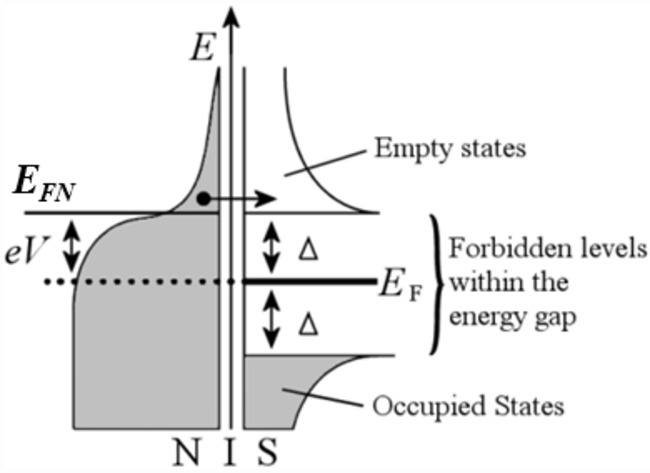
\includegraphics[width = 0.45\textwidth]{energybands}
\caption{The energy-level diagram of an NIS junction. The
superconductor has an energy bandgap of $2 \Delta$ nA bias voltage, $V = \nicefrac{\Delta}{e}$, is applied across the junction, so that only electrons with energy greater than $E_{FN}$ are allowed to tunnel through the insulator into the superconductor. From Pekola \emph{et al.} \cite{Pekola04}.}
\label{fig:energybands}
\end{figure}

\par 
As shown in Fig. \ref{fig:energybands}, only electrons with energies $E>\Delta$
can enter the superconductor, which for voltages $V \leq \nicefrac{\Delta}{e}$,
are hot electrons ($E > E_{FN} $). Cold electrons ($E > E_{FN}$), having $E < \Delta$ are blocked by the energy gap in the superconductor. Each electron removes energy ($E-eV$), which is of order $k_{B} T$, from the metal corresponding to a cooling power of order $ \nicefrac{Ik_{B}T}{e}$ where $I$ is the current through the junction \cite{Nahum94, Fisher99}. The reduction in electron energy corresponds to a lowering of the electron temperature. Maximum cooling power occurs for voltages closely approaching $V = \nicefrac{\Delta}{e}$. For $V > \nicefrac{\Delta}{e}$, cold electrons are also extracted from the normal metal and at high bias the tunneling results in a net negative cooling power i.e. a heat load which is equivalent to Joule heating \cite{Giazotto06}.

\begin{figure}[!t]
\centering
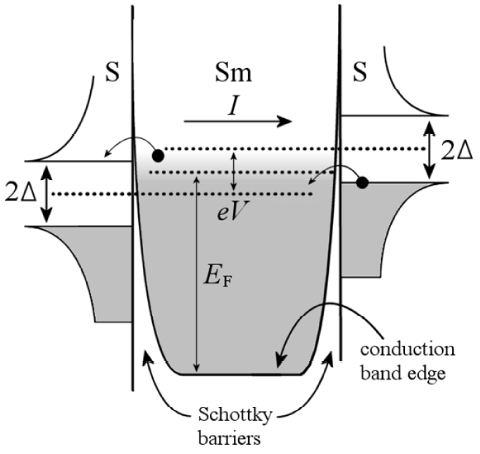
\includegraphics[width = 0.45\textwidth]{SSmS}
\caption{Energy-band diagram illustrating cooling in the S--Sm--S structure. S denotes the superconductor and Sm the semiconductor. $2\Delta$ is the energy gap in the superconductor, $E_{F}$ the Fermi energy of the semiconductor, and $P$ heat flow out of the semiconductor. $V$ is the applied voltage and $I$ is the resulting current. The grey areas denote the Fermi distribution of occupied electron states. From \cite{Savin01}.}
\label{fig:SSmS}
\end{figure}

\par
Small NIS probe junctions are used to measure temperature. The small area increases the tunnel resistance, so that the cooling power of the probe
junction is kept small.

\par 
If $k_{B}T_{e} \ll \Delta$ and $0 \ll eV < \Delta$, the current through an
NIS junction, by thermally activated tunneling, according to \cite{Nahum93} is:

\begin{align}
I(V) &\approx I_{a} \exp \frac{eV - \Delta}{k_{B}T_{e}},
\intertext{such that if the junction is biased with a constant current:}
\frac{dV}{dT_{e}} &\approx \frac{k_{B}}{e} \ln \left( \frac{I}{I_{a}} \right). 
\end{align}
\par 
Hence, the thermometer voltage has a suitably linear dependence on temperature. However, in real devices there is often a deviation from this linear dependence at the lowest temperatures \cite{Nahum94}.

\par 
Savin and co-workers replaced the normal metal with a degenerate semiconductor (Sm), in the arrangement shown in Fig. \ref{fig:SSmS} \cite{Savin01}. Cooling was demonstrated, but not from the technologically important temperature of 300 mK.

\begin{figure}[!t]
\centering
\subfloat[]{
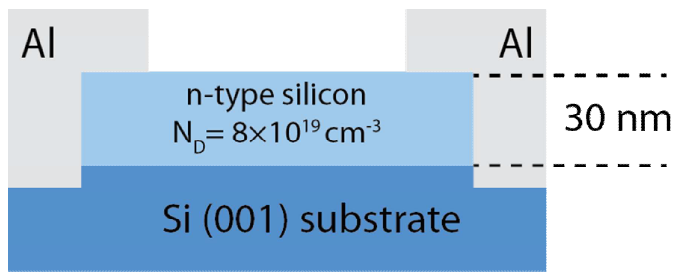
\includegraphics[width=0.45\textwidth]{cross-section}
\label{fig:cross-section}
} \\
\subfloat[]{
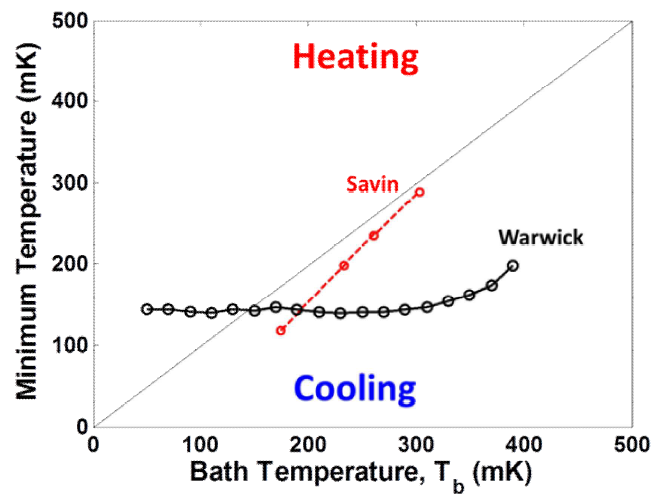
\includegraphics[width=0.45\textwidth]{cooling-heating}
\label{fig:cooling-heating}
}
\caption{(a) Simplified block schematic of silicon-superconductor
tunnel junction cooler; (b) Cooling performance, red symbols -- Savin
\cite{Savin01}; black symbols -- Warwick \cite{Richardson-BullockUP}; above line -� heating regime; below line -- cooling regime.}
\label{fig:x-sec&cooling}
\end{figure}

\par
Fig. \ref{fig:cross-section} shows a block schematic of the Warwick cooler. With this structure we have achieved electron cooling from 300 mK to 150 mK, for the first time \cite{Richardson-BullockUP}, as shown in Fig. \ref{fig:cooling-heating}.

\begin{figure}[!t]
\centering
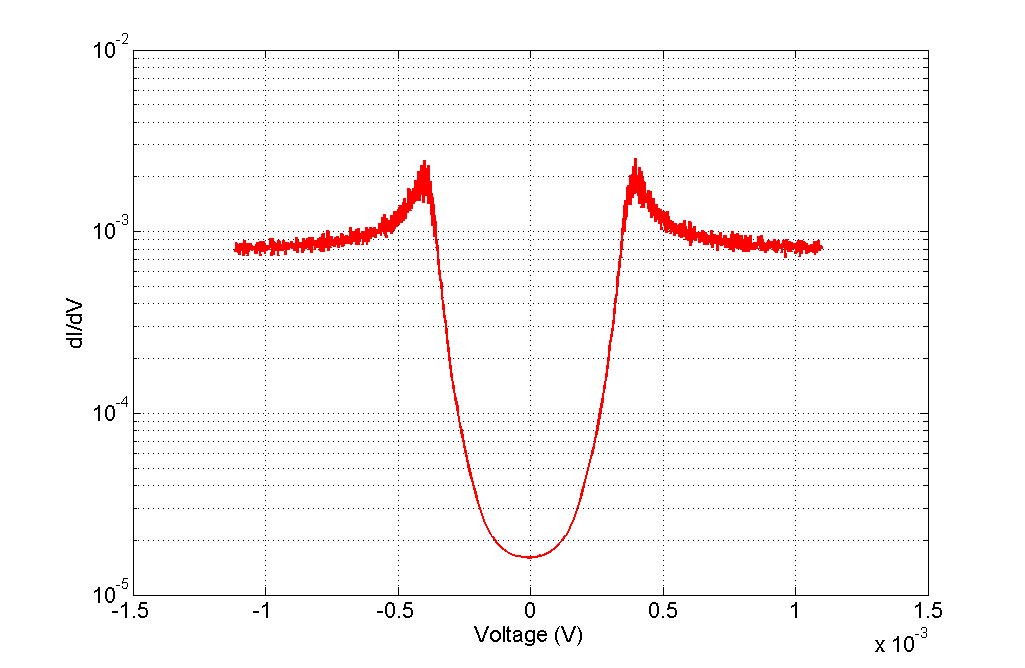
\includegraphics[width=0.45\textwidth]{dIdV}
\caption{Tunneling conductance $\nicefrac{dI}{dV}$ of a typical silicon
superconductor Schottky barrier junction measured at 100 mK. Dynes
parameter, $\Gamma$, is $2 \times 10^{-2}$. From \cite{BrienUP}.}
\label{fig:dIdV}
\end{figure}

\par
An important indicator of cooler performance is the low-temperature Dynes parameter, which is defined as the sub-gap conductance divided by the normal state tunneling conductance, illustrated in Fig. \ref{fig:dIdV}, for a typical Warwick sample \cite{Richardson-BullockUP, BrienUP}.

\par 
Efforts are being made to improve this property of the junction. Further improvements in cooling performance should be possible by engineering the band structure and the scattering processes. Modeling suggests that by using a superconductor of sufficient quality and higher transition temperature and by increasing the Schottky barrier transmissivity, it may be possible to cool from 1 K to below 0.25 K. This would represent a sea-change in cooling, dramatically reducing the complexity required of the mechanical/liquid refrigerator still further. Temperatures of below 100 mK could be accessed by cascading electron coolers using superconductors of different band gaps.


\section{The Cold Electron Bolometer}
Fig. \ref{fig:bolometer&CEBantenna} illustrates the basic principle of the bolometer and how it is implemented in silicon. In our first realization of this concept, we have mounted the silicon in a 150 GHz twin slot antenna, as shown in Fig. \ref{fig:CEB}, using aluminium as the superconductor. In this arrangement, the antenna focusses the radiation in to the silicon, doped n--type at $4 \times 10^{19}$ cm\textsuperscript{-3}, and the associated Schottky junctions serve as the thermometer.

\begin{figure}[!t]
\centering
\subfloat[]{
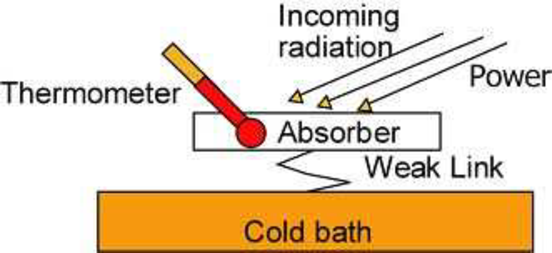
\includegraphics[width=0.38\textwidth]{bolometer}
\label{fig:bolometer}
} \\
\subfloat[]{
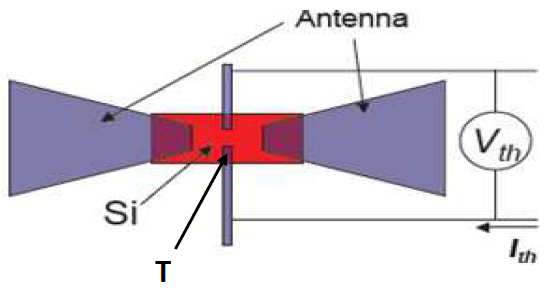
\includegraphics[width=0.38\textwidth]{CEB-antenna}
\label{fig:CEB-antenna}
} \\
\subfloat[]{
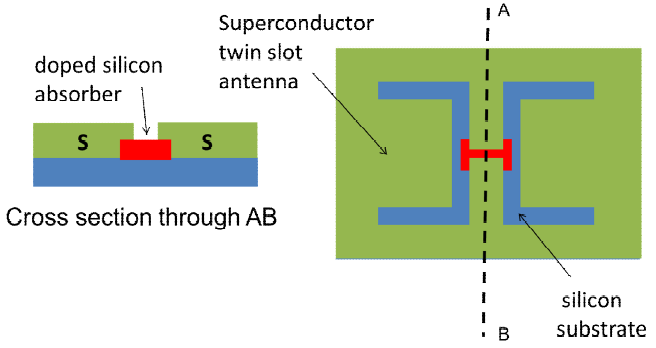
\includegraphics[width=0.45\textwidth]{CEB}
\label{fig:CEB}
}
\caption{(a) Incoming radiation raises the temperature of the absorber. By measuring its temperature, we can deduce the intensity and wavelength of the radiation. (b) An antenna focusses the radiation onto the silicon and the tunnel junction thermometer T is used to measure the ensuing temperature rise. (c) CEB with twin--slot antenna.}
\label{fig:bolometer&CEBantenna}
\end{figure}

\par
Since the junctions pass a current, they also provide significant cooling. To explore this aspect, we refer to the work of Golobev and Kuzmin \cite{Golubev01}, concerning the analogous SINIS bolometer. They calculate that, at the appropriate bias where cooling occurs, there is a pronounced increase in the bolometer responsivity, as shown in Fig. \ref{fig:CEB-cooling}.

\begin{figure}[!t]
\centering
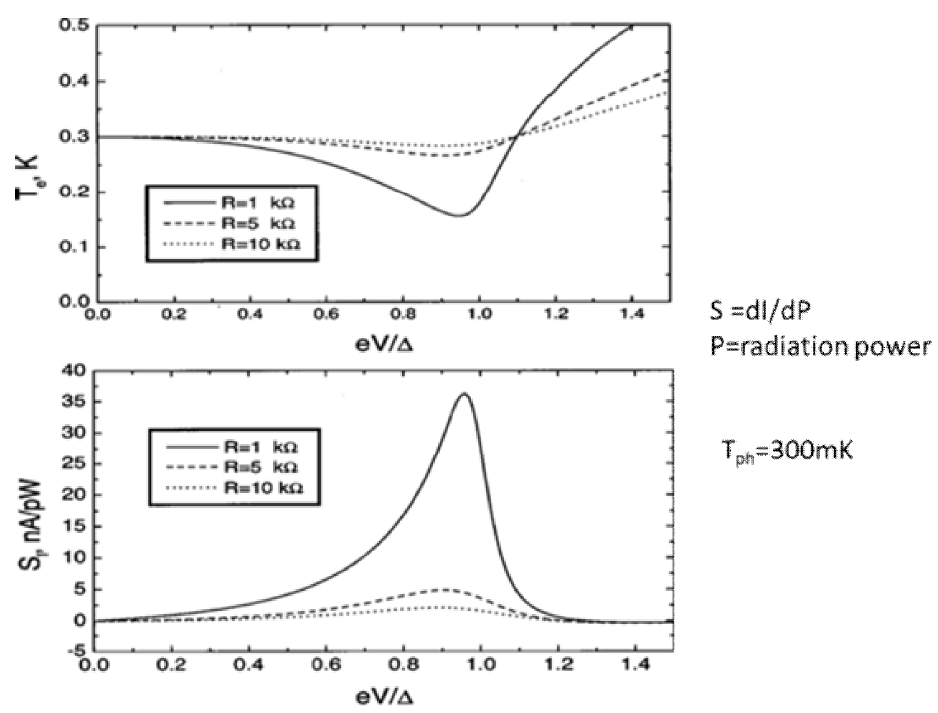
\includegraphics[width=0.45\textwidth]{CEB-cooling}
\caption{Effect of cooling in the SINIS configuration, on the bolometer responsivity. The junctions are biased at constant voltage. $R$ is the tunnel resistance, which determines the cooling power. From \cite{Golubev01}.}
\label{fig:CEB-cooling}
\end{figure}

\par 
Preliminary results \cite{BrienUP} on our bolometer may be explained with reference to this work. In Fig. \ref{fig:Responsivity} we show the response of the silicon bolometer to 150 GHz at different powers. In this case, the bolometer is current biased. The peak responsivity occurs where maximum cooling is expected (at around $\nicefrac{2 \Delta}{e}$) and is of the order $10^{8}$ V/W.

\begin{figure}[!t]
\centering
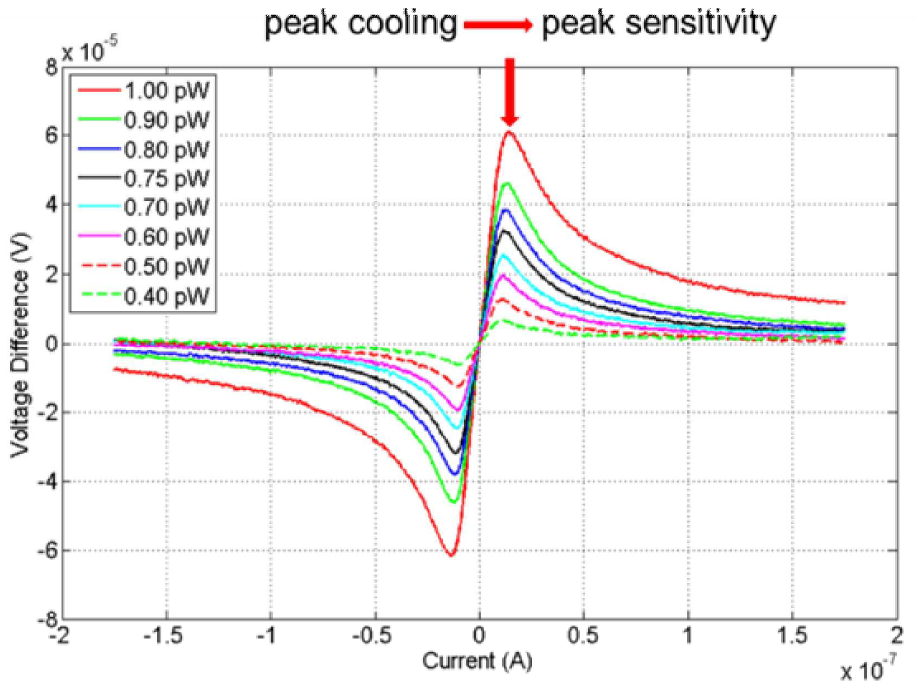
\includegraphics[width=0.45\textwidth]{Responsivity}
\caption{Responsivity of the silicon bolometer versus bias current, for various incident radiation powers. $\Delta V$ is the change in voltage when the radiation source is turned on.}
\label{fig:Responsivity}
\end{figure}

\par 
In Fig. \ref{fig:SINIS-NEP} Golubev and Kuzmin show that the bias dependent cooling in a single tunnel junction model has a beneficial effect on the signal to noise ratio, and by extension the noise equivalent power (NEP) \cite{Golubev01}. The reductions in amplifier and shot noise are associated with the increase in bolometer responsivity at optimum bias. The reduction in phonon noise stems from the fall in electron phonon coupling with electron temperature. Preliminary measurements \cite{BrienUP} on the silicon bolometer show similar behaviour, as seen in Fig. \ref{fig:CEB-NEP}.

\begin{figure}[!t]
\centering
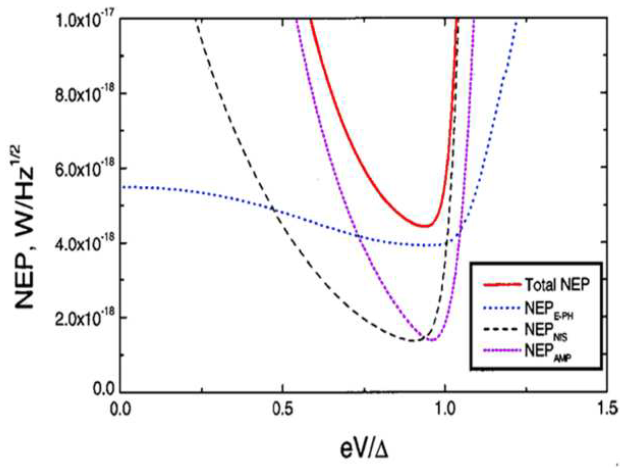
\includegraphics[width=0.45\textwidth]{SINIS-NEP}
\caption{NIS bolometer Noise Equivalent Power in the voltage biased mode for a single junction, showing the effect of cooling on the amplifier current noise, the junction shot noise and the phonon noise. Bath temperature is 300 mK and tunnel resistance $R = 1~k\Omega$. From \cite{Golubev01}.}
\label{fig:SINIS-NEP}
\end{figure}

\begin{figure}[!t]
\centering
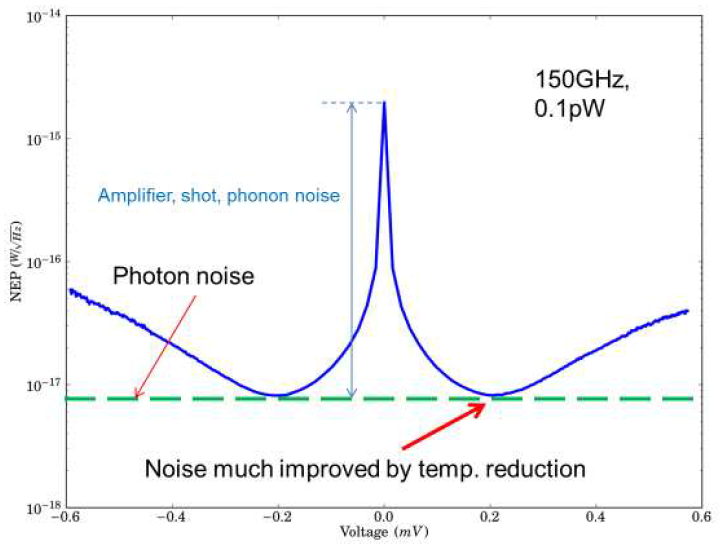
\includegraphics[width=0.45\textwidth]{CEB-NEP}
\caption{Measurements of the NEP of a silicon bolometer at a lattice/bath temperature of 280 mK, and in the presence of 0.1 pW of radiation.}
\label{fig:CEB-NEP}
\end{figure}

\par 
The minimum in NEP occurs at a bias voltage of 0.4 mV, corresponding to maximum electron cooling by the junctions. Since the minimum NEP corresponds to the photon noise, calculated for 0.1 pW of power from the radiation source, we may conclude that the bolometer and electronics noise is much less than $10^{-17}~W/\sqrt{Hz}$.

\section{Conclusions}
We have shown that superconducting tunnel junction coolers may be used to improve the performance of a novel silicon bolometer. 
\newpage 
The applications of this technology are much more wide-ranging than described here. We are currently carrying out research on lattice, or phonon, cooling, which will extend the range of �cooltronic� applications to encompass superconducting transition edge sensors, superconducting tunnel junction photodetectors and superconducting quantum bits.



\bibliographystyle{IEEEtran}
\bibliography{IEEEabrv,Bib}

\end{document}
